\documentclass[editMode]{ufdissertation}\sloppy

%%%%%%%%%%%%%%%%%%%%%%%%%%%%%%%%%%%%%%%%%%%%%%%%%%%%%%%%%%%%%%%%%%%%%%%%%%%%%%%%
%%%                 User Package and Style File loading.
%%%%%%%%%%%%%%%%%%%%%%%%%%%%%%%%%%%%%%%%%%%%%%%%%%%%%%%%%%%%%%%%%%%%%%%%%%%%%%%%

%\usepackage{CustomMacros}%  This is a user macro/style file.

\usepackage{tikz}%       tikz is used by almost everyone, but certainly by me for this.
\usepackage{pgfplots}%   pgfplots is tikz but better.
%\usepackage{amsrefs}%   amsrefs contains the .bibtex style content for mathematician papers.
\usepackage{algorithmic}
\usepackage{xcolor}

%%%%%%%%%%%%%%%%%%%%%%%%%%%%%%%%%%%%%%%%%%%%%%%%%%%%%%%%%%%%%%%%%%%%%%%%%%%%%%%%
%%%                     User Configuration commands
%%%%%%%%%%%%%%%%%%%%%%%%%%%%%%%%%%%%%%%%%%%%%%%%%%%%%%%%%%%%%%%%%%%%%%%%%%%%%%%%

%% Uncomment the relevant line below if you have tables or figures
\haveTablestrue%        Uncomment this if you have tables in your thesis.
\haveFigurestrue%       Uncomment this if you have figures in your thesis.

%%%%%%%%%%%%%%%%%%%%%%%%%%%%%%%%%%%%%%%%%%%%%%%%%%%%%%%%%%%%%%%%%%%%%%%%%%%%%%%%
%%% Below are the commands to set the degree type, department, graduation time, and chair. 
%       Most of these are self-explanatory. 
%       Note: The \chair command takes an optional argument for a co-chair. 
%           So if John was your chair and Jacob was a cochair, you would use \chair[Jacob]{John}.
%           If John was your chair and you had no cochair, you can simply use \chair{John}.
%%%%%%%%%%%%%%%%%%%%%%%%%%%%%%%%%%%%%%%%%%%%%%%%%%%%%%%%%%%%%%%%%%%%%%%%%%%%%%%%

\title{An Autonomous Method for Measuring 3D Joint Kinematics from 2D Xray Images}%  Put your title here.

\degreeType{Doctorate of Philosophy}%   Official name of your degree; e.g. "Doctorate of Philosophy."
\major{Mechanical Engineering}%                    Your official Department
\author{Andrew James Jensen}%                  Your Name
\thesisType{Dissertation}%              Dissertation (PhD) or Thesis (Masters)
\degreeYear{2022}%                      Intended graduation year (not the year you submit the thesis)
\degreeMonth{December}%                   Month of graduation should be May, August, or December.
\chair{Scott Banks}%                   Chair and Cochair (see comment block above).


%%%%%%%%%%%%%%%%%%%%%%%%%%%%%%%%%%%%%%%%%%%%%%%%%%%%%%%%%%%%%%%%%%%%%%%%%%%%%%%%
%%% For each of the following, type in the name of the file that contains each section. 
%       They are assumed to be tex files, but if they aren't, the command takes an optional argument for the extension.
%       So, you could load dedication.tex as your dedication file using \setDedicationFile{dedication}
%       You could load dedication.txt instead with \setDedicationFile[txt]{dedication}.
%       NOTE: For some compilers, they may or may not add a .tex to the end of the file automatically.
%           If you get a "couldn't find dedication.tex.tex" type error, try the command with an empty optional argument,
%           e.g. \setDedicationFile[]{dedication}
%%%
%%%%%%%%%%%%%%%%%%%%%%%%%%%%%%%%%%%%%%%%%%%%%%%%%%%%%%%%%%%%%%%%%%%%%%%%%%%%%%%%

%%% These are REQUIRED sections; easiest to do via these commands.

\setDedicationFile{./src/dedicationFile}%                 Dedication Page
\setAcknowledgementsFile{./src/acknowledgementsFile}%     Acknowledgements Page
\setAbstractFile{./src/abstractFile}%                     Abstract Page (This should only include the abstract itself)
\setReferenceFile{./src/referenceFile}{amsplain}%         References. First argument is your bibtex source file
%                                                       the second argument is your bibtex style file.
\setBiographicalFile{./src/biographyFile}%                Biography file of the Author (you).

%%% These are NOT required, so only use them if you actually need/have them.

\setAbbreviationsFile{./src/abbreviations}%           Abbreviations Page
%\setAppendixFile{appendix}%                     Appendix Content; hyperlinking might be weird.
%\multipleAppendixtrue%                          Uncomment this if you have more than one appendix, 
%                                                   comment it if you have only one appendix.


%%%%%%%                     End of File Assignment
%%%%%%%%%%%%%%%%%%%%%%%%%%%%%%%%%%%%%%%%%%%%%%%%%%%%%%%%%%%%%%%%%%%%%%%%%%%%%%%%

\begin{document}
%%%% Here you just need to include/input your actual work. 
%       The above files (dedication, acknowledgment, title page, etc, etc) will all be added for you 
%       using the files you assigned above. 
%       If you want to input the above files manually you can comment out the \setFILE command above 
%       and use \input or \include here. Generally you want to use \include to get your pagebreak.
%       NOTE: If you input manually you will have to do some/all the formatting manually.



\chapter{Introduction}

\section{A subsection of the introduction}

\subsection{another subsection of the introduction}

This sheet is part of the introduction test test
\chapter{Literature Review}

This is the introduction to the literature review that I am going to write

\begin{equation}
    \frac{hello}{goodbye}
\end{equation}


\chapter{EXAMPLES OF EDITOR/Author TOOLS, TABLES, AND IMAGES}% Notice that we can use chapter/section etc breaks in the master file if we want, and then use \input instead of \include to avoid unneccessary page breaks.
%\section{Example of using the authorRemark and editorRemark}
If you don't see any blue or red type under this line, then you almost certainly need to include the optional ``editMode" to the document class. Thus your document class (first line) should read \verb|\documentclass[editMode]{ufdissertation}|.

\authorRemark{Test! This is a remark written by the author, to themselves, for review purposes. It will be suppressed unless editMode is used in the class options.}

\editorRemark{This is an editor's remark, written by an editor in-line so that they can write into the content itself with something easy to see. But the remark will be suppressed unless editMode is used in the class options.

To get this remark to go away, simply remove ``editMode" from the documentclass options at the top of the user's tex-file. This also removes the blue Author Remarks.
}%     Stuff about using editorRemark and authorRemark commands
%\section{Table Examples}% Notice that the section command needs to be included in the file somewhere. The \include command will not generate chapter or section breaks automatically.
You may notice that some tables get moved outside of where you placed them. This is because \LaTeX{} is a little too helpful when it comes to placement of `float' types; which includes tables and figures. You can get around this by using the ``H" parameter in the table environment, or the `multiFigure' environment described in the ``adding graphics section"; ie section \ref{Sec:addingGraphics}

\begin{table}[H]
\caption[An example of a table caption in the incorrect place.]{This table is located in the correct section because it uses the ``H" optional parameter in the table environment, unlike the next tables which have been helpfully moved by \LaTeX{} to the next page, which places them inside the section.You should also make a note that the caption command is placed after the table itself, which means the caption occurs after the table. The graduate school requires tables to have captions placed {before} the actual table data, so the caption command should be located before the table data. See the next table for an example.}
\begin{tabular}{llcr}
\hline Some    & Data  & Goes  & Here\\ \hline
Some    & Data  & Goes  & Here\\
Some    & Data  & Goes  & Here\\
Some    & Data  & Goes  & Here\\
\hline
\end{tabular}

\end{table}

\begin{table}[]
\caption[A proper table caption location]{Notice that this caption is included above the table data, as per the graduate school requirements. Also note that the caption itself has a short version in the ``List of Tables" which is achieved by using the optional argument of the caption command. See the file source code directly to see the example. Unfortunately, since we did not use the ``H" parameter in the table environment, this table was placed \textit{after} the next section heading, which is almost certainly not where an author would have wanted it.}
%\begin{center}
\begin{tabularx}{\textwidth}{XXXX}
\hline Some    & Data  & Goes  & Here\\ \hline
Some    & Data  & Goes  & Here\\
Some    & Data  & Goes  & Here\\
Some    & Data  & Goes  & Here\\
\hline
\end{tabularx}
%\end{center}

\end{table}

\section{Very Long Tables}

There are two approaches to inputting very long tables. You can do it manually, or you can do it using the longtables package. Here we include an example of both. Table \ref{tbl1} is done manually, whereas \ref{tbl2} is done using the longtables package.

\begin{table}[H]
\caption{Feasible triples for highly variable Grid, MLMMH.} \label{tbl1}
\begin{tabularx}{6.5 in}{r l X}
\hline {{Time (s)}} & {{Triple chosen}} & {{Other feasible triples}} \\ \hline
0 & (1, 11, 13725) & (1, 12, 10980), (1, 13, 8235), (2, 2, 0), (3, 1, 0) \\
2745 & (1, 12, 10980) & (1, 13, 8235), (2, 2, 0), (2, 3, 0), (3, 1, 0) \\
5490 & (1, 12, 13725) & (2, 2, 2745), (2, 3, 0), (3, 1, 0) \\
8235 & (1, 12, 16470) & (1, 13, 13725), (2, 2, 2745), (2, 3, 0), (3, 1, 0) \\
10980 & (1, 12, 16470) & (1, 13, 13725), (2, 2, 2745), (2, 3, 0), (3, 1, 0) \\
13725 & (1, 12, 16470) & (1, 13, 13725), (2, 2, 2745), (2, 3, 0), (3, 1, 0) \\
16470 & (1, 13, 16470) & (2, 2, 2745), (2, 3, 0), (3, 1, 0) \\
19215 & (1, 12, 16470) & (1, 13, 13725), (2, 2, 2745), (2, 3, 0), (3, 1, 0) \\
21960 & (1, 12, 16470) & (1, 13, 13725), (2, 2, 2745), (2, 3, 0), (3, 1, 0) \\
24705 & (1, 12, 16470) & (1, 13, 13725), (2, 2, 2745), (2, 3, 0), (3, 1, 0) \\
27450 & (1, 12, 16470) & (1, 13, 13725), (2, 2, 2745), (2, 3, 0), (3, 1, 0) \\
30195 & (2, 2, 2745) & (2, 3, 0), (3, 1, 0) \\
32940 & (1, 13, 16470) & (2, 2, 2745), (2, 3, 0), (3, 1, 0) \\
35685 & (1, 13, 13725) & (2, 2, 2745), (2, 3, 0), (3, 1, 0) \\
38430 & (1, 13, 10980) & (2, 2, 2745), (2, 3, 0), (3, 1, 0) \\
41175 & (1, 12, 13725) & (1, 13, 10980), (2, 2, 2745), (2, 3, 0), (3, 1, 0) \\
43920 & (1, 13, 10980) & (2, 2, 2745), (2, 3, 0), (3, 1, 0) \\
46665 & (2, 2, 2745) & (2, 3, 0), (3, 1, 0) \\
49410 & (2, 2, 2745) & (2, 3, 0), (3, 1, 0) \\
52155 & (1, 12, 16470) & (1, 13, 13725), (2, 2, 2745), (2, 3, 0), (3, 1, 0) \\
54900 & (1, 13, 13725) & (2, 2, 2745), (2, 3, 0), (3, 1, 0) \\
57645 & (1, 13, 13725) & (2, 2, 2745), (2, 3, 0), (3, 1, 0) \\
60390 & (1, 12, 13725) & (2, 2, 2745), (2, 3, 0), (3, 1, 0) \\
63135 & (1, 13, 16470) & (2, 2, 2745), (2, 3, 0), (3, 1, 0) \\
65880 & (1, 13, 16470) & (2, 2, 2745), (2, 3, 0), (3, 1, 0) \\
68625 & (2, 2, 2745) & (2, 3, 0), (3, 1, 0) \\
71370 & (1, 13, 13725) & (2, 2, 2745), (2, 3, 0), (3, 1, 0) \\
74115 & (1, 12, 13725) & (2, 2, 2745), (2, 3, 0), (3, 1, 0) \\
76860 & (1, 13, 13725) & (2, 2, 2745), (2, 3, 0), (3, 1, 0) \\
79605 & (1, 13, 13725) & (2, 2, 2745), (2, 3, 0), (3, 1, 0) \\
82350 & (1, 12, 13725) & (2, 2, 2745), (2, 3, 0), (3, 1, 0) \\
\hline
\end{tabularx}
\end{table}

\begin{table}[h!t!]
\begin{tabularx}{6.5 in}{r l X}
\multicolumn{3}{l}{Table \ref{tbl1}. Continued}\\%
\hline {{Time (s)}} & {{Triple chosen}} & {{Other feasible triples}} \\ \hline
85095 & (1, 12, 13725) & (1, 13, 10980), (2, 2, 2745), (2, 3, 0), (3, 1, 0) \\
87840 & (1, 13, 16470) & (2, 2, 2745), (2, 3, 0), (3, 1, 0) \\
90585 & (1, 13, 16470) & (2, 2, 2745), (2, 3, 0), (3, 1, 0) \\
93330 & (1, 13, 13725) & (2, 2, 2745), (2, 3, 0), (3, 1, 0) \\
96075 & (1, 13, 16470) & (2, 2, 2745), (2, 3, 0), (3, 1, 0) \\
98820 & (1, 13, 16470) & (2, 2, 2745), (2, 3, 0), (3, 1, 0) \\
101565 & (1, 13, 13725) & (2, 2, 2745), (2, 3, 0), (3, 1, 0) \\
104310 & (1, 13, 16470) & (2, 2, 2745), (2, 3, 0), (3, 1, 0) \\
107055 & (1, 13, 13725) & (2, 2, 2745), (2, 3, 0), (3, 1, 0) \\
109800 & (1, 13, 13725) & (2, 2, 2745), (2, 3, 0), (3, 1, 0) \\
112545 & (1, 12, 16470) & (1, 13, 13725), (2, 2, 2745), (2, 3, 0), (3, 1, 0) \\
115290 & (1, 13, 16470) & (2, 2, 2745), (2, 3, 0), (3, 1, 0) \\
118035 & (1, 13, 13725) & (2, 2, 2745), (2, 3, 0), (3, 1, 0) \\
120780 & (1, 13, 16470) & (2, 2, 2745), (2, 3, 0), (3, 1, 0) \\
123525 & (1, 13, 13725) & (2, 2, 2745), (2, 3, 0), (3, 1, 0) \\
126270 & (1, 12, 16470) & (1, 13, 13725), (2, 2, 2745), (2, 3, 0), (3, 1, 0) \\
129015 & (2, 2, 2745) & (2, 3, 0), (3, 1, 0) \\
131760 & (2, 2, 2745) & (2, 3, 0), (3, 1, 0) \\
134505 & (1, 13, 16470) & (2, 2, 2745), (2, 3, 0), (3, 1, 0) \\
137250 & (1, 13, 13725) & (2, 2, 2745), (2, 3, 0), (3, 1, 0) \\
139995 & (2, 2, 2745) & (2, 3, 0), (3, 1, 0) \\
142740 & (2, 2, 2745) & (2, 3, 0), (3, 1, 0) \\
145485 & (1, 12, 16470) & (1, 13, 13725), (2, 2, 2745), (2, 3, 0), (3, 1, 0)\\%
148230 & (2, 2, 2745) & (2, 3, 0), (3, 1, 0) \\
150975 & (1, 13, 16470) & (2, 2, 2745), (2, 3, 0), (3, 1, 0) \\
153720 & (1, 12, 13725) & (2, 2, 2745), (2, 3, 0), (3, 1, 0) \\
156465 & (1, 13, 13725) & (2, 2, 2745), (2, 3, 0), (3, 1, 0) \\
159210 & (1, 13, 13725) & (2, 2, 2745), (2, 3, 0), (3, 1, 0) \\
161955 & (1, 13, 16470) & (2, 2, 2745), (2, 3, 0), (3, 1, 0) \\
164700 & (1, 13, 13725) & (2, 2, 2745), (2, 3, 0), (3, 1, 0) \\
\hline
\end{tabularx}
\end{table}

Alternatively, compared to the previous example where we used manual breaks to break the table, we can let LaTeX do this for us, as well as taking care of any recurrent headers and footers, utilizing the \verb|\longtable| command,\footnote{note that the longtable environment is not in a table environment; putting it inside a table environment will stop it from correctly page breaking as needed.} as follows:

\newpage

\begin{longtable}[h!t!]{p{0.6in}p{1in}p{4.4in}}
    \caption{Duplicate of Previous table, using longtables environment.}\label{tbl2}\\% Default caption at top of table
    \hline {{Time (s)}} & {{Triple chosen}} & {{Other feasible triples}}\\ \hline \endfirsthead% The top row of the first page
    \hline\endfoot%         This line should always be included; it includes a line at the end of the table on every page.
    \caption*{Table 4-4. Continued} \\% This caption is added to every page after the first as per the \endhead next line.
    \hline{{Time (s)}} & {{Triple chosen}} & {{Other feasible triples}}\\ \hline \endhead%
%                                                               Everything between \endfoot and \endhead here is added at
%                                                                   the top of the table on every page except the first;
%                                                                   The first page is an exception because we have defined a
%                                                                   \endfirsthead row already which superceeds \endhead.
0 & (1, 11, 13725) & (1, 12, 10980), (1, 13, 8235), (2, 2, 0), (3, 1, 0)\\
2745 & (1, 12, 10980) & (1, 13, 8235), (2, 2, 0), (2, 3, 0), (3, 1, 0) \\
5490 & (1, 12, 13725) & (2, 2, 2745), (2, 3, 0), (3, 1, 0) \\
8235 & (1, 12, 16470) & (1, 13, 13725), (2, 2, 2745), (2, 3, 0), (3, 1, 0) \\
10980 & (1, 12, 16470) & (1, 13, 13725), (2, 2, 2745), (2, 3, 0), (3, 1, 0) \\
13725 & (1, 12, 16470) & (1, 13, 13725), (2, 2, 2745), (2, 3, 0), (3, 1, 0) \\
16470 & (1, 13, 16470) & (2, 2, 2745), (2, 3, 0), (3, 1, 0) \\
19215 & (1, 12, 16470) & (1, 13, 13725), (2, 2, 2745), (2, 3, 0), (3, 1, 0) \\
21960 & (1, 12, 16470) & (1, 13, 13725), (2, 2, 2745), (2, 3, 0), (3, 1, 0) \\
24705 & (1, 12, 16470) & (1, 13, 13725), (2, 2, 2745), (2, 3, 0), (3, 1, 0) \\
27450 & (1, 12, 16470) & (1, 13, 13725), (2, 2, 2745), (2, 3, 0), (3, 1, 0) \\
30195 & (2, 2, 2745) & (2, 3, 0), (3, 1, 0) \\
32940 & (1, 13, 16470) & (2, 2, 2745), (2, 3, 0), (3, 1, 0) \\
35685 & (1, 13, 13725) & (2, 2, 2745), (2, 3, 0), (3, 1, 0) \\
38430 & (1, 13, 10980) & (2, 2, 2745), (2, 3, 0), (3, 1, 0) \\
41175 & (1, 12, 13725) & (1, 13, 10980), (2, 2, 2745), (2, 3, 0), (3, 1, 0) \\
43920 & (1, 13, 10980) & (2, 2, 2745), (2, 3, 0), (3, 1, 0) \\
46665 & (2, 2, 2745) & (2, 3, 0), (3, 1, 0) \\
49410 & (2, 2, 2745) & (2, 3, 0), (3, 1, 0) \\
52155 & (1, 12, 16470) & (1, 13, 13725), (2, 2, 2745), (2, 3, 0), (3, 1, 0) \\
54900 & (1, 13, 13725) & (2, 2, 2745), (2, 3, 0), (3, 1, 0) \\
57645 & (1, 13, 13725) & (2, 2, 2745), (2, 3, 0), (3, 1, 0) \\
60390 & (1, 12, 13725) & (2, 2, 2745), (2, 3, 0), (3, 1, 0) \\
63135 & (1, 13, 16470) & (2, 2, 2745), (2, 3, 0), (3, 1, 0) \\
65880 & (1, 13, 16470) & (2, 2, 2745), (2, 3, 0), (3, 1, 0) \\
68625 & (2, 2, 2745) & (2, 3, 0), (3, 1, 0) \\
71370 & (1, 13, 13725) & (2, 2, 2745), (2, 3, 0), (3, 1, 0) \\
74115 & (1, 12, 13725) & (2, 2, 2745), (2, 3, 0), (3, 1, 0) \\
76860 & (1, 13, 13725) & (2, 2, 2745), (2, 3, 0), (3, 1, 0) \\
79605 & (1, 13, 13725) & (2, 2, 2745), (2, 3, 0), (3, 1, 0) \\
82350 & (1, 12, 13725) & (2, 2, 2745), (2, 3, 0), (3, 1, 0) \\
85095 & (1, 12, 13725) & (1, 13, 10980), (2, 2, 2745), (2, 3, 0), (3, 1, 0) \\
87840 & (1, 13, 16470) & (2, 2, 2745), (2, 3, 0), (3, 1, 0) \\
90585 & (1, 13, 16470) & (2, 2, 2745), (2, 3, 0), (3, 1, 0) \\
93330 & (1, 13, 13725) & (2, 2, 2745), (2, 3, 0), (3, 1, 0) \\
96075 & (1, 13, 16470) & (2, 2, 2745), (2, 3, 0), (3, 1, 0) \\
98820 & (1, 13, 16470) & (2, 2, 2745), (2, 3, 0), (3, 1, 0) \\
101565 & (1, 13, 13725) & (2, 2, 2745), (2, 3, 0), (3, 1, 0) \\
104310 & (1, 13, 16470) & (2, 2, 2745), (2, 3, 0), (3, 1, 0) \\
107055 & (1, 13, 13725) & (2, 2, 2745), (2, 3, 0), (3, 1, 0) \\
109800 & (1, 13, 13725) & (2, 2, 2745), (2, 3, 0), (3, 1, 0) \\
112545 & (1, 12, 16470) & (1, 13, 13725), (2, 2, 2745), (2, 3, 0), (3, 1, 0) \\
115290 & (1, 13, 16470) & (2, 2, 2745), (2, 3, 0), (3, 1, 0) \\
118035 & (1, 13, 13725) & (2, 2, 2745), (2, 3, 0), (3, 1, 0) \\
120780 & (1, 13, 16470) & (2, 2, 2745), (2, 3, 0), (3, 1, 0) \\
123525 & (1, 13, 13725) & (2, 2, 2745), (2, 3, 0), (3, 1, 0) \\
126270 & (1, 12, 16470) & (1, 13, 13725), (2, 2, 2745), (2, 3, 0), (3, 1, 0) \\
129015 & (2, 2, 2745) & (2, 3, 0), (3, 1, 0) \\
131760 & (2, 2, 2745) & (2, 3, 0), (3, 1, 0) \\
134505 & (1, 13, 16470) & (2, 2, 2745), (2, 3, 0), (3, 1, 0) \\
137250 & (1, 13, 13725) & (2, 2, 2745), (2, 3, 0), (3, 1, 0) \\
139995 & (2, 2, 2745) & (2, 3, 0), (3, 1, 0) \\
142740 & (2, 2, 2745) & (2, 3, 0), (3, 1, 0) \\
145485 & (1, 12, 16470) & (1, 13, 13725), (2, 2, 2745), (2, 3, 0), (3, 1, 0)\\%
148230 & (2, 2, 2745) & (2, 3, 0), (3, 1, 0) \\
150975 & (1, 13, 16470) & (2, 2, 2745), (2, 3, 0), (3, 1, 0) \\
153720 & (1, 12, 13725) & (2, 2, 2745), (2, 3, 0), (3, 1, 0) \\
156465 & (1, 13, 13725) & (2, 2, 2745), (2, 3, 0), (3, 1, 0) \\
159210 & (1, 13, 13725) & (2, 2, 2745), (2, 3, 0), (3, 1, 0) \\
161955 & (1, 13, 16470) & (2, 2, 2745), (2, 3, 0), (3, 1, 0) \\
164700 & (1, 13, 13725) & (2, 2, 2745), (2, 3, 0), (3, 1, 0) \\
\end{longtable}

%    Stuff about using Tables.
%\section{Examples of Adding Graphics}
\label{Sec:addingGraphics}
All of the below code with subfigures A-Z was generated with:
\begin{verbatim}
\begin{multiFigure}
\addFigure{0.3}{./theworld.png}
\addFigure{0.2}{./theworld.png}
\addFigure{0.4}{./theworld.png}
\addFigure[Z]{0.6}{./theworld.png}
\captionof{figure}[This is a test caption.]{This is a test caption. 
This text has the bit for the whole figure.  Meanwhile, subfigure A is weird 
looking map. Subfigure B is a smaller map. And Subfigure C 
is a bigger but still weird looking map. 
Moreover, I can override the map, which is why Z is 
another weird map that came after map C.}
\end{multiFigure}
\end{verbatim}
Note that \LaTeX{} can be fickle when it comes to placing figures relative to text near the figure. Specifically, the ``Figure" environment is a `float' type, which is placed somewhere ``nearby" where it appears in the text, which can be pretty frustrating. For this reason we have circumvented the `float' part of the figure in order to allow more control over the figure placement. 

If one uses the \verb|\begin{figure}\end{figure}| construction, the figure may appear in a odd place, whereas you can use the \verb|\begin{multiFigure}\end{multiFigure}| even with only 1 figure, to force placement to work. When using multiFigure captions need to be placed using the command \verb|\captionof{<NAME>}[<LIST-ENTRY>]{<CAPTION>}| where NAME is the type of caption, LIST-ENTRY is what appears in the `List of' at the beginning of the thesis, and CAPTION is the actual caption. For single image figures, it will be better to use the \verb|\begin{figure}\end{figure}| construction was the Graduate Editorial Office does not need a letter-label, for a figure with only one image. 

\begin{flushleft}
    \begin{multiFigure}
        \begin{center}
            \addFigure{0.3}{graphics/theworld.png}
            \addFigure{0.2}{graphics/theworld.png}
            \addFigure{0.4}{graphics/theworld.png}
            \addFigure[Z]{0.6}{graphics/theworld.png}
        \end{center}
\captionof{figure}[This is my shortened caption for my Table of Contents]{This is a test caption. This text has the bit for the whole figure. Meanwhile, subfigure A is weird looking map. Subfigure B is a smaller map. And Subfigure C is a bigger but still weird looking map. Moreover, I can override the map, which is why Z is another weird map that came after map C.}
\end{multiFigure}
\end{flushleft}


\begin{figure}[h!]
    \begin{center}
        \includegraphics[width=0.9\textwidth]{graphics/theworld.png}
    \end{center}
     \caption[This is my shortened caption for my Table of Contents] {This is a super-long caption to make sure that the caption in the list-of section is correctly single space with the blank white line between captions. That being said, you should probably always use the list-entry optional argument in the captionof command to write a shorter caption instead of this nonsense.}
\end{figure}

\section{A Note on Graphics}
The command \verb|\addFigure| in the multiFigure environment, and/or the command \verb|\includegraphics| will take almost every type of graphic file currently in use as of the writing of this template. The only notable exception is the bitmap, ie .bmp file. Most software won't save to bitmap without specifically requesting it at this point, but if you have generated a .bmp file you can load it in most any graphic editor (eg MSpaint or photoshop) and save it as a different file type, such as .PNG which is significantly smaller file size as well. Note that the commands typically require the file extension to be included, and it is case sensitive. Thus in the above \verb|\addFigure{0.2}{./theworld.png}| works but \verb|\addFigure{0.2}{./theworld.PNG}| would error and \verb|\addFigure{0.2}{./theworld}| may or may not work depending on which specific TeX editor you are using.

\section{Placement Specifiers}

Floats are used to allow LaTeX to handle figures while maintaining the best possible presentation. However, there may be times when you disagree, and a typical example is with its positioning of figures. The placement specifier parameter exists as a compromise, and its purpose is to give the author a greater degree of control over where certain floats are placed. 


\begin{table}[H]
\caption{Specifier Table}
\begin{tabular}{l p{14cm} }
\hline
Specifier & Permission \\ \hline
h & Place the float here, i.e., approximately at the same point it occurs in the source text (however, not exactly at the spot) \\
\\
t & Position at the top of the page.  \\
\\
b & Position at the bottom of the page.  \\
\\
p & Put on a special page for floats only.  \\
\\
! & Override internal parameters LaTeX uses for determining "good" float positions. \\
\\
H & Places the float at precisely the location in the LaTeX code. \\
\hline
\end{tabular}
\end{table}

An example of a specifier parameter is shown below to force a figure into place where it is mentioned in text: 

\begin{verbatim}
\begin{figure}[h!]
    \begin{center}
        \includegraphics[width=0.9\textwidth]{./theworld.png}
    \end{center}
     \caption[My short caption.]{My full caption in curly brackets.}
\end{figure}
\end{verbatim}%    Stuff about using Images.

%\chapter{SUMMARY AND CONCLUSIONS} \label{conclusion}

\section{Non Porttitor Tellus}

Aliquam molestie sed urna quis convallis. Aenean nibh eros, aliquam non eros in, tempus lacinia justo. In magna sapien, blandit a faucibus ac, scelerisque nec purus. Praesent fermentum felis nec massa interdum, vel dapibus mi luctus. Cras id fringilla mauris. Ut molestie eros mi, ut hendrerit nulla tempor et. Pellentesque tortor quam, mattis a scelerisque nec, euismod et odio. Mauris rhoncus metus sit amet risus mattis, eu mattis sem interdum.

\subsection{Nam Arcu Magna}
Semper vel lorem eu, venenatis ultrices est. Nam aliquet ut erat ac scelerisque. Maecenas ut molestie mi. Phasellus ipsum magna, sollicitudin eu ipsum quis, imperdiet cursus turpis. Etiam pretium enim a fermentum accumsan. Morbi vel vehicula enim.

\subsection{Nam Arcu Magna}
Semper vel lorem eu, venenatis ultrices est. Nam aliquet ut erat ac scelerisque. Maecenas ut molestie mi. Phasellus ipsum magna, sollicitudin eu ipsum quis, imperdiet cursus turpis. Etiam pretium enim a fermentum accumsan. Morbi vel vehicula enim.

\subsubsection{Ut pellentesque velit sede}
 Placerat cursus. Integer congue urna non massa dictum, a pellentesque arcu accumsan. Nulla posuere, elit accumsan eleifend elementum, ipsum massa tristique metus, in ornare neque nisl sed odio. Nullam eget elementum nisi. Duis a consectetur erat, sit amet malesuada sapien. Aliquam nec sapien et leo sagittis porttitor at ut lacus. Vivamus vulputate elit vitae libero condimentum dictum. Nulla facilisi. Quisque non nibh et massa ullamcorper iaculis.\cite{BigRudin}
 
 \subsubsection{Ut pellentesque velit sede}
 Placerat cursus. Integer congue urna non massa dictum, a pellentesque arcu accumsan. Nulla posuere, elit accumsan eleifend elementum, ipsum massa tristique metus, in ornare neque nisl sed odio. Nullam eget elementum nisi. Duis a consectetur erat, sit amet malesuada sapien. Aliquam nec sapien et leo sagittis porttitor at ut lacus. Vivamus vulputate elit vitae libero condimentum dictum. Nulla facilisi. Quisque non nibh et massa ullamcorper iaculis.\cite{BigRudin}
 
 \section{Non Porttitor Tellus}

Aliquam molestie sed urna quis convallis. Aenean nibh eros, aliquam non eros in, tempus lacinia justo. In magna sapien, blandit a faucibus ac, scelerisque nec purus. Praesent fermentum felis nec massa interdum, vel dapibus mi luctus. Cras id fringilla mauris. Ut molestie eros mi, ut hendrerit nulla tempor et. Pellentesque tortor quam, mattis a scelerisque nec, euismod et odio. Mauris rhoncus metus sit amet risus mattis, eu mattis sem interdum.

% Modified from old template.



\end{document}

